\chapter{Prototype}
Chapter \ref{chapter:gep_neat} explored the theoretical foundation of GEP-NEAT, a hybrid algorithm that integrates the expressive capabilities of Gene Expression Programming (GEP) with the innovation-preserving strategies of NEAT. This chapter shifts focus to the prototype implementation of GEP-NEAT, translating the conceptual framework into a functional system.

\parbreak\noindent Section \ref{sec:proto_introduction} introduces the design rationale behind the construction of the algorithm, outlining key architectural decisions, Section \ref{sec:proto_proto} then presents the full implementation details, covering the core components and mechanisms that drive GEP-NEAT. Following the implementation, the prototype is applied to a series of benchmark problems, with results and visual illustrations discussed in Section \ref{sec:proto_results}. This chapter concludes in Section \ref{sec:proto_conclusion}, summarising the outcomes and reflecting on the effectiveness of the prototype.

\section{Introduction}\label{sec:proto_introduction}
With reference to Chapter \ref{chapter:research_methodology}, this study adopts the Design Science Research (DSR) paradigm, which, as previously discussed, is centered on the creation of innovative artifacts that contribute meaningfully to the existing body of scientific knowledge within a specific domain. DSR emphasises both the design and rigorous evaluation of artifacts, ensuring that they are not only novel but also effective in addressing real-world problems.

\parbreak\noindent As noted by \cite{olivier2009information}, one of the early limitations of the DSR paradigm was the absence of a clearly defined set of operational steps or standardised tool. To address this, Olivier proposed a more structured approach, particularly emphasising the role of conceptual modeling. He argued that models can take various forms, such as descriptive, metaphorical, formal, etc., and may be expressed using principles, scientific notation, or visual languages, depending on research context.

\parbreak\noindent In the context of this research, where the artifact is a genetic algorithm-based system, the implementation naturally lends itself to programmatic modeling. Therefore, the design of the GEP-NEAT prototype is supported by the use of UML class diagrams and sequence diagrams. The class diagram provides a clear and structured representation of the system's components, their relationships, and responsibilities, effectively serving as a blueprint for the artifact's construction. The sequence diagram, on the other hand, captures the control flow and interaction logic between components, offering a high-level view of the algorithm's runtime behaviour. Based on these models, the algorithm is implemented using a programming language, translating the conceptual design into a functional prototype. This approach ensures that the artifact remains aligned with its theoretical foundation while being practically executable and testable.

\parbreak\noindent The evaluation of the prototype is conducted through both quantitative and qualitative methods, in line with DSR's emphasis on rigorous validation. Quantitative evaluation involves measuring the algorithm's performance using standard metrics such as accuracy, precision, convergence speed, and efficiency (\cite{gregar2023research}). These metrics provide objective insights into how well the artifact performs across different problem domains. Complementing this, the qualitative evaluation focuses on the artifact's structural and functional qualities, including modularity, scalability, and innovative design features. As \cite{olivier2009information} emphasises, qualitative insights are essential for assessing how well the prototype aligns with its conceptual model and whether it contributes meaningfully to the broader knowledge base.

\parbreak\noindent In this research, the GEP-NEAT prototype is applied to a variety of problem scenarios to assess its generalisability and effectiveness. The results of these experiments are analysed in relation to the research questions posed earlier in the dissertation. While some questions are directly answered through empirical results, others are addressed through interpretive analysis and discussion, providing a comprehensive understanding of the artifact's capabilities and limitations.

\section{GEP-NEAT Prototype}\label{sec:proto_proto}
Since this research follows the Design Science Research (DSR) methodology, and draws on the insights provided by \cite{olivier2009information}, the hybrid algorithm introduced in Chapter \ref{chapter:gep_neat} is formally architected using programmatic modeling techniques. Specifically, the system design is captured through a class diagram, shown in Figure \ref{fig:proto_class_diagram}, which serves as a blueprint for the prototype's implementation.

\parbreak\noindent The central component of the system is the chromosome, which represents a candidate solution to the problem. Each chromosome is composed of symbols that follow the structure of Karva notation, a linear representation format commonly used in Gene Expression Programming. These symbols are categorized into three distinct types:
\begin{itemize}
    \item \textbf{Function Symbol}: Represents an operator drawn from the function set. Each function symbol stores its arity (i.e., the number of inputs it accepts), the associated activation function, a flag indicating whether bias is enabled, and the bias value itself.
    \item \textbf{Terminal Symbol}: Represents an input value drawn from the terminal set, typically corresponding to raw data or constants.
    \item \textbf{Weight Symbol}: Represents an index used to access values from the weight lookup array.
\end{itemize}

\parbreak\noindent The activation function associated with each function symbol is selected from a predefined set housed within the activation function class. Notably, each function symbol within a chromosome can point to a different activation function, allowing the system to learn and adapt which activation behaviours are most suitable for a given task.

\parbreak\noindent The chromosome itself is composed of six key attributes:
\begin{itemize}
    \item \textbf{Neuron Genes}: A list of neuron genes, each containing a sequence of symbols that form a valid expression tree. In GEP-NEAT, neuron genes are used to encode multiple outputs. For example, a classification task requiring decisions for red, green, and blue would have three neuron genes, each representing a distinct output pathway.
    \item \textbf{Weight Genes}: A list of weight genes corresponding to the neuron genes. Each weight gene contains symbols that reference weight indices, which are used to access corresponding values in the weight lookup array.
    \item \textbf{Weight Lookup Genes}: A list of values that serve as the actual weights. The weight gene symbols act as index accessors to retrieve values from this array.
    \item \textbf{Fitness}: The raw fitness score of the chromosome, measuring its performance on the given task.
    \item \textbf{Adjusted Fitness}: A normalised fitness score used during speciation and selection.
    \item \textbf{Innovation Number Composition}: A list of dictionaries that tracks the innovation numbers composition associated with each neuron gene. This structure records the arrangement of subtrees and their corresponding weights, enabling comparison due to the fact that the same subtree configurations can be represented differently by changing order.
\end{itemize}

\parbreak\noindent Beyond the chromosome, the system includes several supporting classes:
\begin{itemize}
    \item \textbf{Genetic Operators}: A collection of methods responsible for modifying chromosomes through mutation, crossover, transposition, and other evolutionary mechanisms.
    \item \textbf{Config}: A configuration class that stores all user-defined hyperparameters, summarised in Table \ref{table:proto_hyper}.
    \item \textbf{Algorithm}: The core class that orchestrates the evolutionary process, including initialisation, evaluation, selection, and reproduction.
\end{itemize}

\parbreak\noindent The sequence diagram, shown in Figure \ref{fig:proto_sequence_diagram}, illustrates the flow of control throughout the system. Functions marked with the \textit{@} symbol denote auxiliary logic, embedded directly for simplicity but intended to be modularised in future iterations. These auxiliary functions can be extracted into standalone components to improve maintainability and clarity.

\parbreak\noindent The prototype is implemented in Python, chosen for its readability, extensive ecosystem of libraries (including tools like Graphviz for visualising expression trees), and widespread adoption in scientific computing. The program begins with the user configuring the system via the Config class, setting hyperparameters as outlined in Table \ref{table:proto_hyper}. Once initialised, the Python application executes a series of function calls that follow the logical flow depicted in the framework diagram (Figure \ref{fig:gep_neat_framework}).

\parbreak\noindent To aid comprehension, headers are included in the sequence diagram to align specific stages of execution with corresponding steps in the framework. Upon completion, the program outputs a variety of visualisations, including performance metrics (such as fitness versus generations), and the phenotype of the best-evolved expression, rendered using Graphviz.

\begin{xltabular}{\textwidth}{|l|X|l|}
\hline
\rowcolor[HTML]{F8CECC} 
\textbf{Hyperparameter}             & \textbf{Description}                                                                                                      & \textbf{Example Value} \\ \hline
\endfirsthead
%
\endhead
%
Problem                             & Problem that GEP-NEAT is applied to                                                                                       & XOR                    \\ \hline
Meme Influence Decay Rate           & The rate at which the meme influence value decays over generations. Higher values equates to forgetting the meme quicker. & 0.9                    \\ \hline
Number of Runs                      & The number of times the algorithm is executed from scratch, each time starting with a newly initialised population.       & 10                     \\ \hline
Number of Generations               & The number of evolutionary cycles the algorithm runs within a single execution.                                           & 50                     \\ \hline
Head Size                           & The number of symbols within the head portion of the expression string.                                                   & 3                      \\ \hline
Weight Lookup Size                  & The size of the weight lookup array.                                                                                      & 10                     \\ \hline
Weight Lookup Range                 & The range of values which the weight lookup array must confirm to.                                                        & {[}-2, 2{]}            \\ \hline
Population Size                     & The number of candidate solutions within every evolutionary cycle.                                                        & 100                    \\ \hline
Number of Elite Individuals         & The number of best individuals that survive during every evolutionary cycle.                                              & 2                      \\ \hline
Mutation Neuron Rate                & The rate at which a neuron gene is mutated.                                                                               & 0.064                  \\ \hline
Mutation Weight Rate                & The rate at which a weight gene is mutated.                                                                               & 0.05                   \\ \hline
Mutation Weight Lookup Rate         & The rate at which a weight lookup value is mutated.                                                                       & 0.04                   \\ \hline
Inversion Neuron Rate               & The rate at which a neuron gene is inverted between two target sites.                                                     & 0.10                   \\ \hline
Inversion Weight Rate               & The rate at which a weight gene is inverted between two target sites.                                                     & 0.08                   \\ \hline
IS Transposition Rate               & The rate at which a neuron gene has an IS element transposed to a random target site.                                     & 0.10                   \\ \hline
IS Transposition Element Length     & The length that the IS element of the neuron transposition must conform to.                                               & {[}1, 2{]}             \\ \hline
Weight Transposition Rate           & The rate at which a weight gene has an IS element transposed to a random target site.                                     & 0.1                    \\ \hline
Weight Transposition Element Length & The length that the IS element of the weight transposition must conform to.                                               & {[}2, 4{]}             \\ \hline
RIS Transposition Rate              & The rate at which a neuron gene has an IS element transposed to the root of the expression string.                        & 0.05                   \\ \hline
RIS Transposition Element Length    & The length that the IS element of the RIS transposition must conform to.                                                  & {[}3{]}                \\ \hline
MIIST Transposition Rate            & The rate at which a neuron gene has an IS element of the top rated innovation number transposed to a random target site.  & 0.2                    \\ \hline
Gene Transposition Rate             & The rate at which an entire gene domain is transposed to another.                                                         & 0.01                   \\ \hline
One-point Recombination Rate        & The rate at which two individuals recombine using a one-point strategy.                                                   & 0.5                    \\ \hline
Two-point Recombination Rate        & The rate at which two individuals recombine using a two-point strategy.                                                   & 0.6                    \\ \hline
Bias Toggle Rate                    & The rate at which the bias is activated within a randomly chosen function symbol within an expression string.             & 0.5                    \\ \hline
Bias Mutation Rate                  & The rate at which the bias value of a randomly chosen function symbol is mutated.                                         & 0.1                    \\ \hline
Bias Range                          & The range in which the bias values must conform to.                                                                       & {[}-1.5, 1.5{]}        \\ \hline
C1 Coefficient                      & The importance of the non-matching genes in calculating the compatibility distance between two individuals.               & 0.8                    \\ \hline
C2 Coefficient                      & The importance of the weight differences in calculating the compatibility distance between two individuals.               & 0.2                    \\ \hline
Compatibility Threshold             & The threshold at which individuals may be classified as being part of the same species.                                   & 1.2                    \\ \hline
Number of Domains                   & The number of domains within the chromosome.                                                                              & 1                      \\ \hline
Maximum Fitness                     & The maximum fitness that the chromosome can achieve as a requisite to terminate prematuraley.                             & 100                    \\ \hline
Function Set                        & The set from which a function symbol can be drawn from.                                                                   & \{Q, D, T\}            \\ \hline
Terminal Set                        & The set from which a terminal symbol can be drawn from.                                                                   & \{a, b\}               \\ \hline
Number of Episodes                  & The number of episodes a candidate solution should be evaluated in (during simulation based tasks)                        & 10                     \\ \hline
\caption{Hyperparameters of GEP-NEAT alongside a description and example}\label{table:proto_hyper}
\end{xltabular}

\newpage
\thispagestyle{empty}
\begin{landscape}
\begin{figure}[H] % Use [H] to suppress floating and place the figure/table exactly where it is specified in the text
	\centering % Horizontally center the figure on the page
	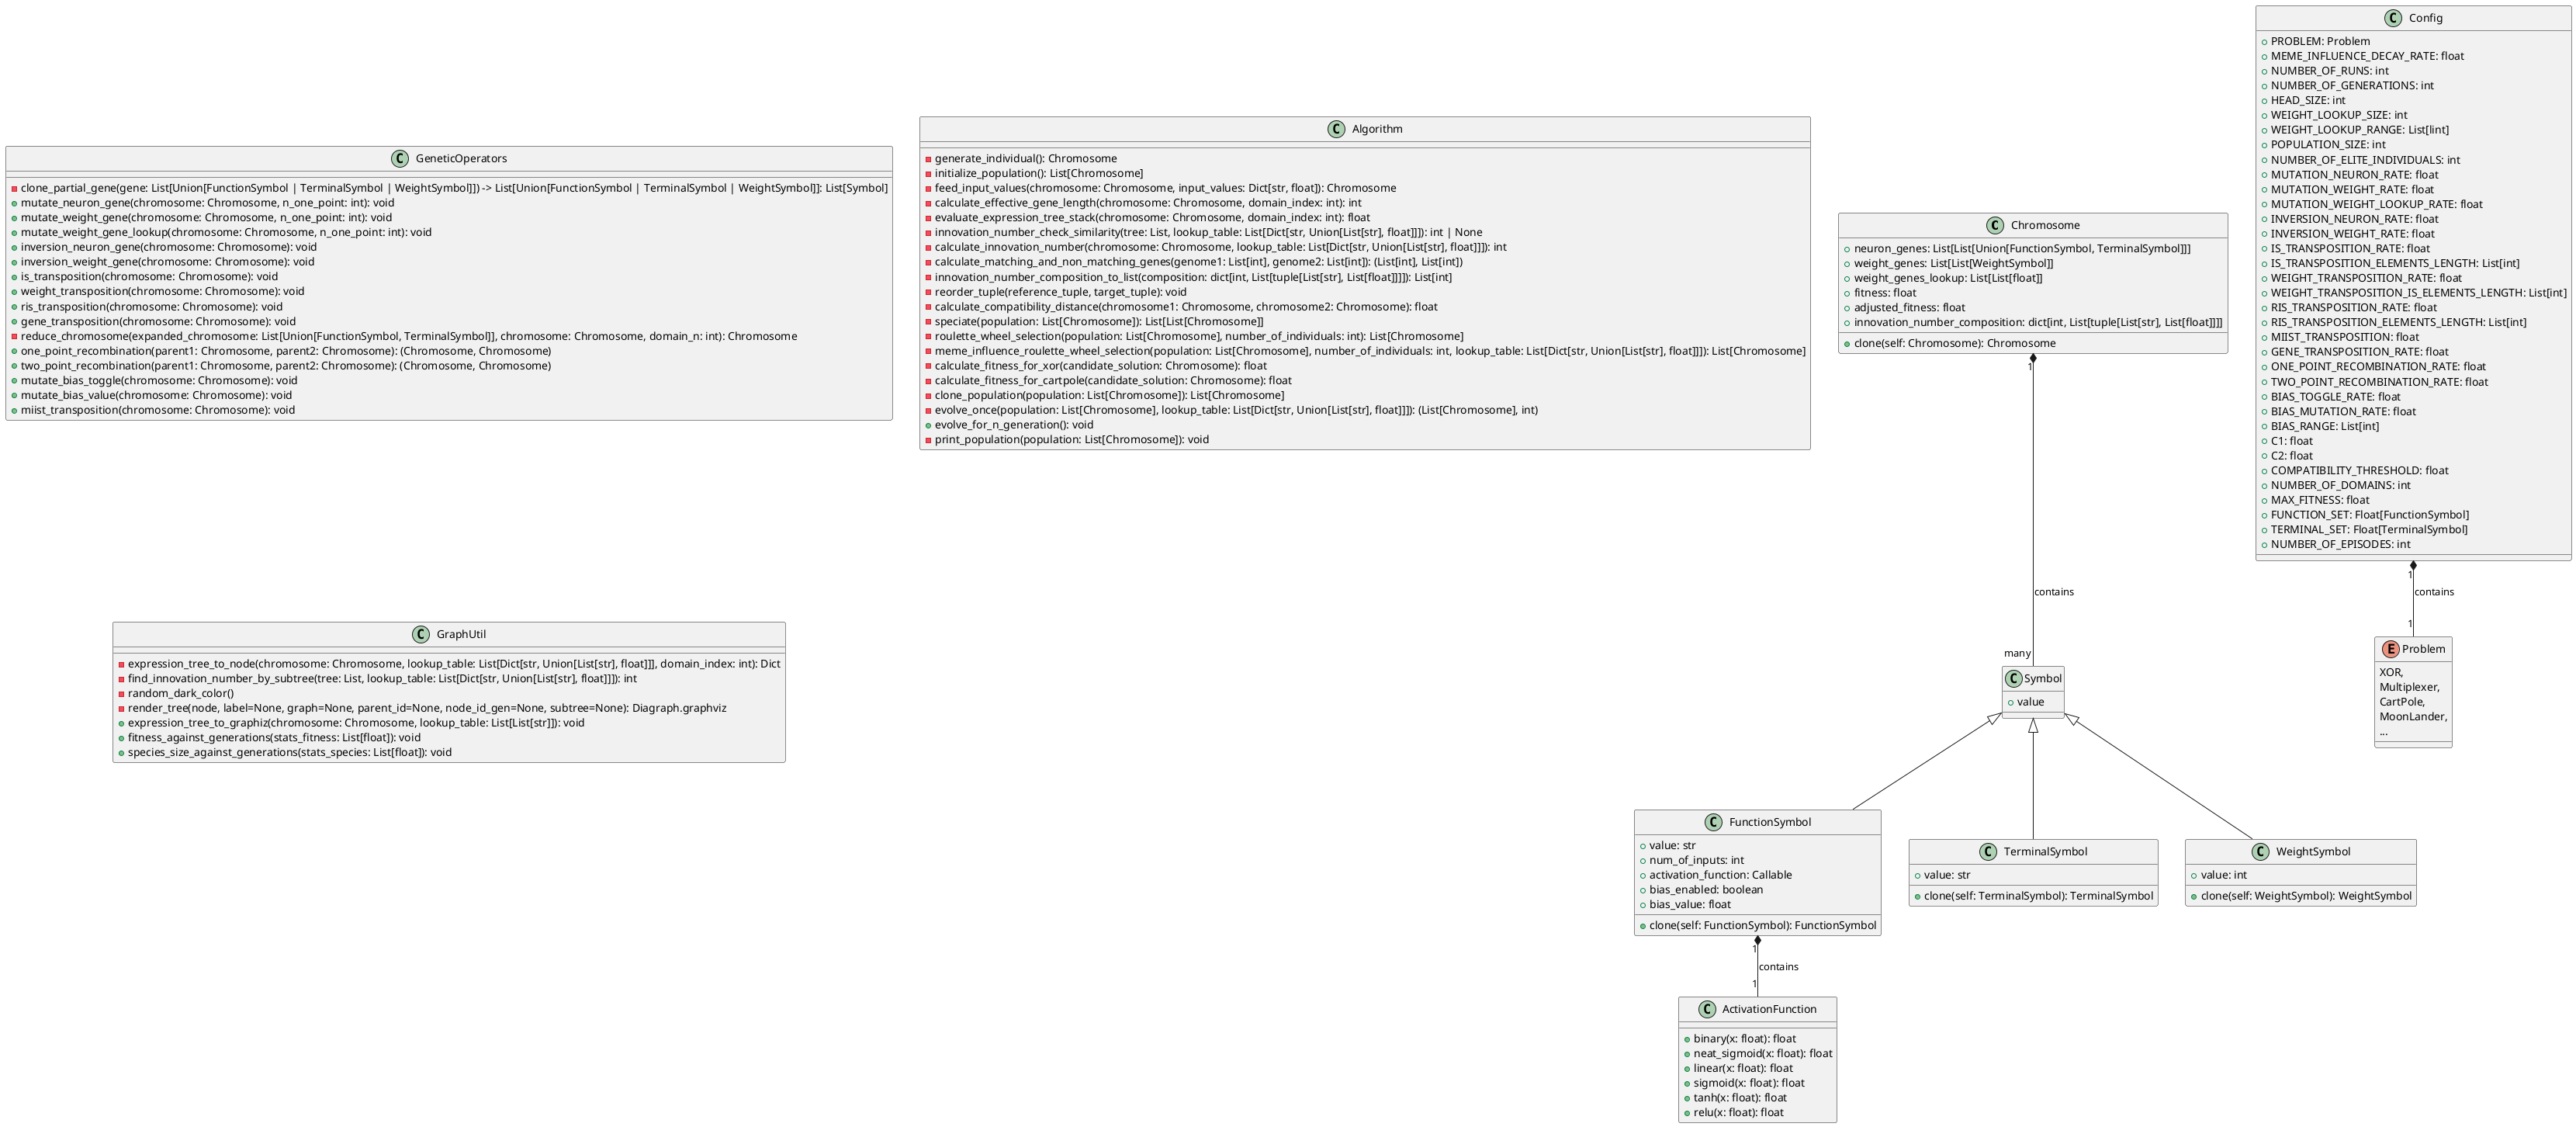
\includegraphics[width=\linewidth]{PlantUml/class_diagram.png} % Include the figure image
	\caption{GEP-NEAT Class Diagram (created using PlantUML)}
	\label{fig:proto_class_diagram} % Unique label used for referencing the figure in-text
\end{figure}
\end{landscape}

\begin{figure}[H] % Use [H] to suppress floating and place the figure/table exactly where it is specified in the text
	\centering % Horizontally center the figure on the page
	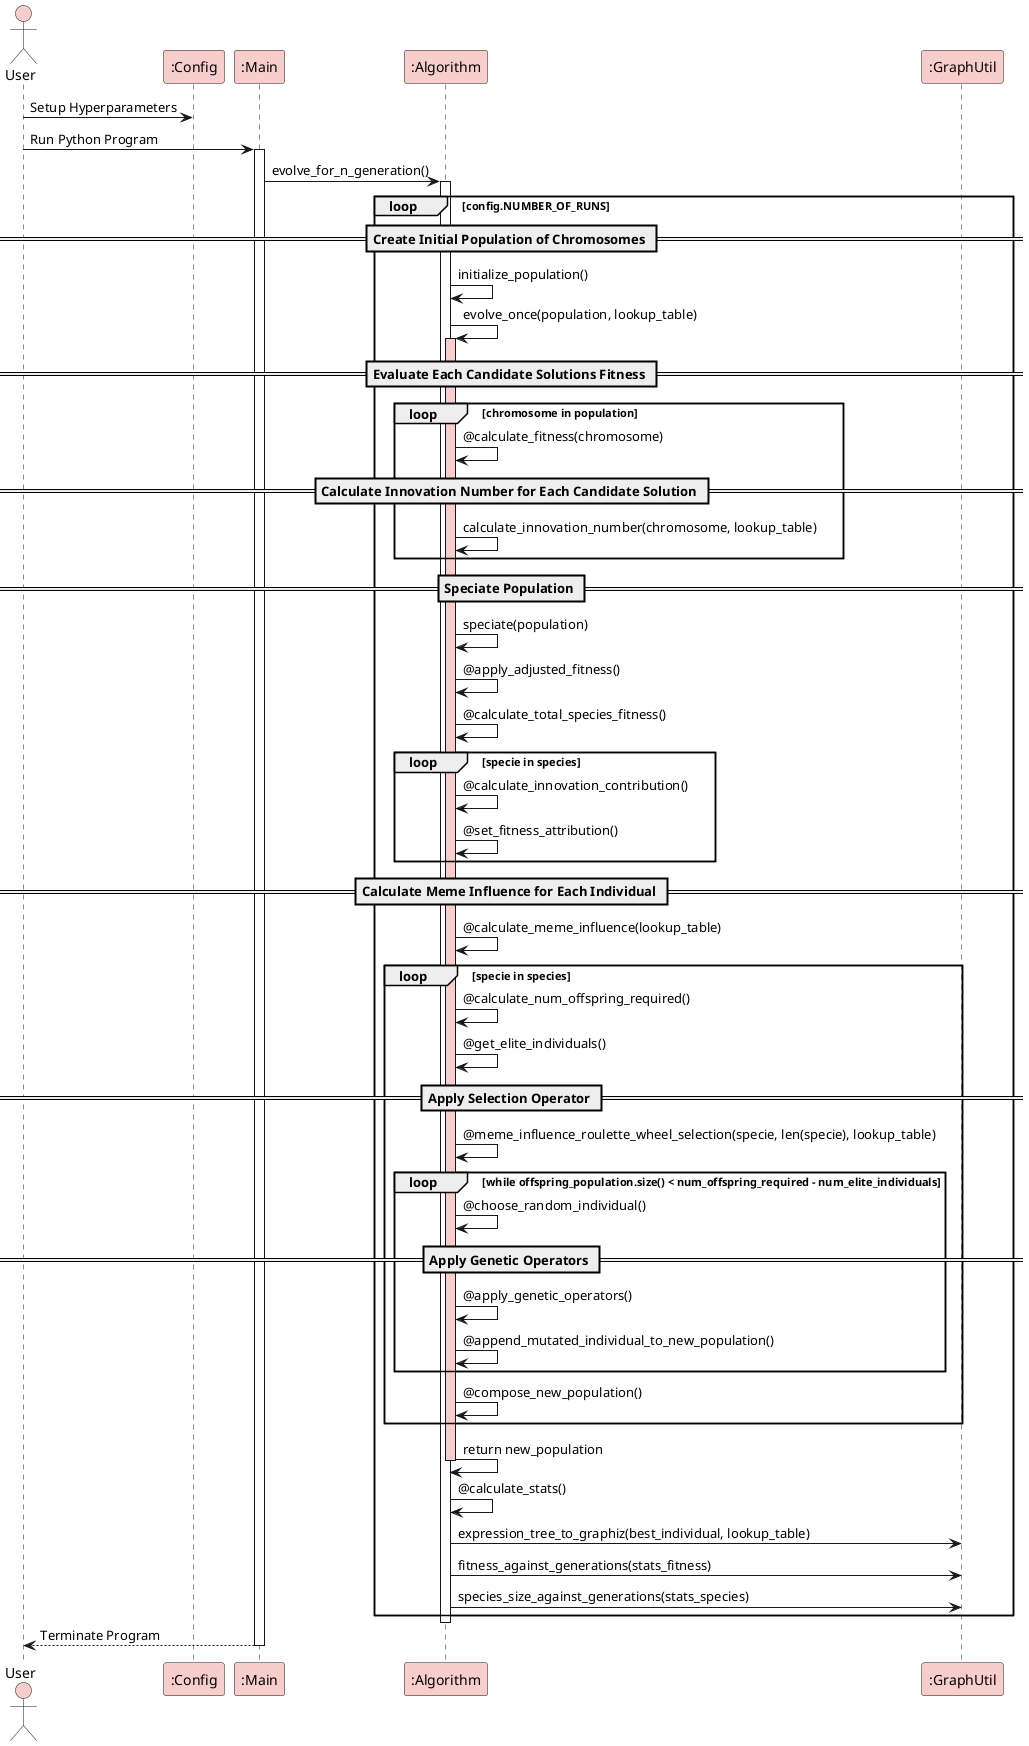
\includegraphics[width=0.80\textwidth]{PlantUml/sequence_diagram.png} % Include the figure image
	\caption{GEP-NEAT Sequence Diagram (created using PlantUML)}
	\label{fig:proto_sequence_diagram} % Unique label used for referencing the figure in-text
\end{figure}

\section{Results}\label{sec:proto_results}

\section{Conclusion}\label{sec:proto_conclusion}
